\hypertarget{laurel-hardy}{%
\section{Laurel \& Hardy}\label{laurel-hardy}}

\begin{figure}[!ht]
  \begin{adjustwidth}{-\oddsidemargin-1in}{-\rightmargin}
    \centering
    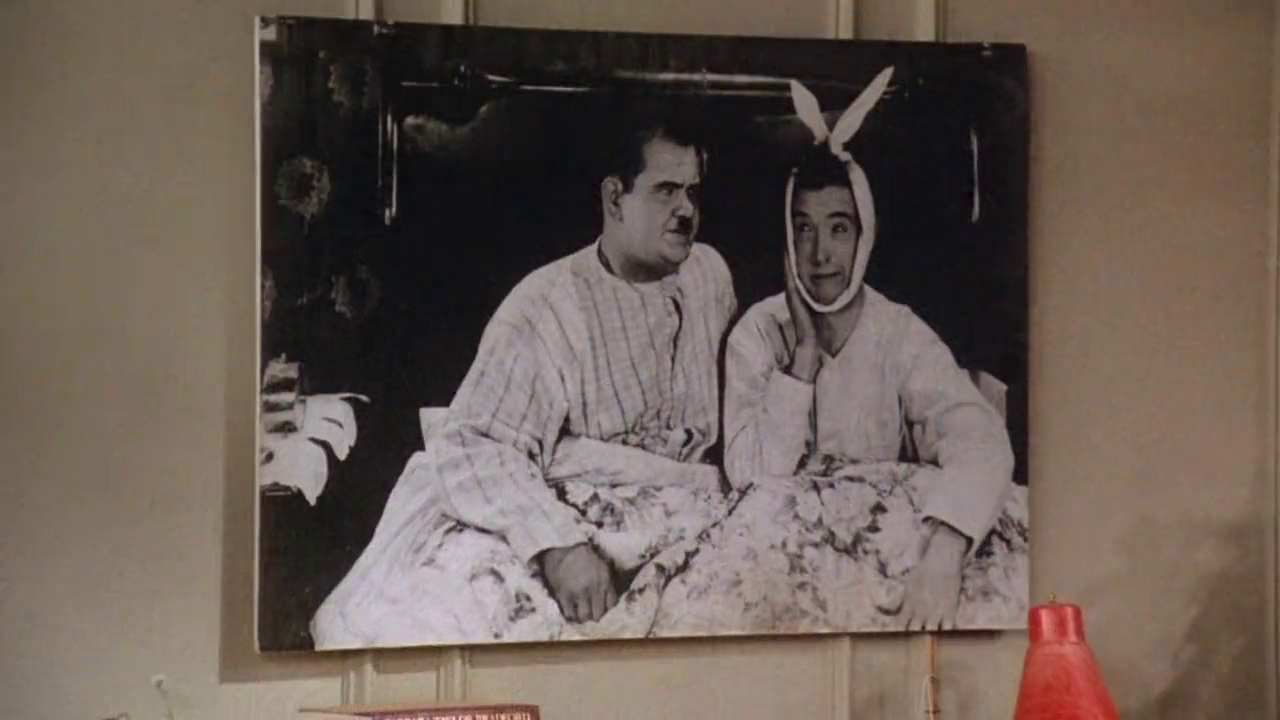
\includegraphics[trim={0 7cm 0 2cm,}, clip, width=\paperwidth]{./S01/img/3/laurel-and-hardy.png}
    % \caption{Laurel & Hardy\label{fig:laurel-hardy}}
  \end{adjustwidth}
\end{figure}

No apartamento de Joey e Chandler, enquanto ensaiam para a audição, um
poster de \emph{Laurel \& Hardy} aparece na sala de estar. Esses
personagens são conhecidos no Brasil como \emph{O Gordo e o Magro} e
fizeram cerca de 106 filmes juntos, entre curtas-metragem sonoros e
mudos e filmes.\footnote{\sloppy Laurel \& Hardy - Site oficial. \url{http://www.laurel-and-hardy.com/}}

\hypertarget{grand-jury-secrets}{%
\section{Grand Jury Secrets}\label{grand-jury-secrets}}

\begin{figure}[!ht]
  \begin{adjustwidth}{-\oddsidemargin-1in}{-\rightmargin}
    \centering
    
\includegraphics[trim={0 6cm 0 3cm,}, clip, width=\paperwidth]{./S01/img/3/grand-jury-secrets.png}
    % \caption{Grand Jury Secrets\label{fig:grand-jury-secrets}}
  \end{adjustwidth}
\end{figure}

\saveparinfos
\noindent
\begin{minipage}[c]{0.5\textwidth}\useparinfo

\emph{Grand Jury Secrets} (1939) é um filme de drama e mistério
americano. Conta a história de um repórter inescrupuloso que obtém
notícias através de um rádio escondido na sala de um júri, onde seu
irmão trabalha como advogado. O repórter é sequestrado e escapa devido
sua capacidade de transmitir sua situação.\footnote{\sloppy BFI. \url{https://www.bfi.org.uk/films-tv-people/4ce2b6ab720c8}}
\footnote{\sloppy Loving The Classics. \url{https://www.lovingtheclassics.com/by-title/g/grand-jury-secrets-1939.html}}
\footnote{\sloppy IMDB. \url{https://www.imdb.com/title/tt0031390/}}

\end{minipage}\hfill
\begin{minipage}[c]{0.5\textwidth}

\begin{figure}
  \centering
  \begin{tikzpicture}
    \node [inner sep=0pt] at (0,0) {
      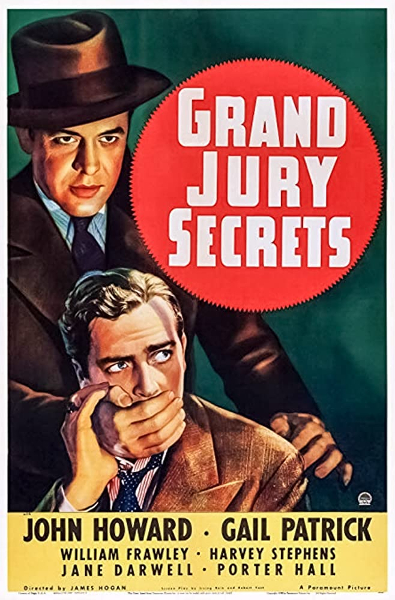
\includegraphics[width=0.7\textwidth,keepaspectratio]{./S01/img/3/grand-jury-secrets-poster.jpg}
    };
    \draw [white, rounded corners=\ClipSep, line width=\ClipSep]
    (current bounding box.north west) --
    (current bounding box.north east) --
    (current bounding box.south east) --
    (current bounding box.south west) -- cycle
    ;
    \end{tikzpicture}
    \caption{Grand Jury Secrets poster\label{fig:grand-jury-secrets-poster}}
\end{figure}

\end{minipage}

\hypertarget{there-was-a-crooked-man}{%
\section{There was a crooked
man\ldots{}}\label{there-was-a-crooked-man}}

\begin{figure}[!ht]
  \begin{adjustwidth}{-\oddsidemargin-1in}{-\rightmargin}
    \centering
    
\includegraphics[trim={0 7cm 0 2cm,}, clip, width=\paperwidth]{./S01/img/3/crooked-man.png}
    % \caption{There was a crooked man\label{fig:there-was-a-crooked-man}}
  \end{adjustwidth}
\end{figure}

\begin{tcolorbox}[enhanced,center upper,
    drop fuzzy shadow southeast, boxrule=0.3pt,
    lower separated=false, breakable,
    colframe=black!30!dialogoBorder,colback=white]
\begin{minipage}[c]{0.16\linewidth}
  \raisebox{\dimexpr-\height+\ht\strutbox\relax}{
    \centering 
\includegraphics[width=1.4cm]{./assets/img/phoebe.png}
  }
   & \centering \scriptsize{Phoebe}
\end{minipage}
\hfill
\begin{minipage}[c]{0.8\linewidth}
  \textbf{- From the nursery rhyme. 'There was a crooked man, Who had a crooked smile, Who lived in a shoe, For a... while...'}\\
  - Da musiquinha. 'Havia um cara de sorriso torto. E morava no sapato, por um... tempo...
\end{minipage}
\end{tcolorbox}

Enquanto os amigos discutem o quanto Alan é legal, Phoebe o compara com
o homem no sapato, que, como Joey notou, tem um sorisso torto. A
``musiquinha'' ou canção de ninar é \emph{There Was a Crooked Man} (C.
1840) de origem desconhecida.\footnote{Alchin, Linda Kathryn.
  \emph{Secret History of Nursery Rhymes.} Linda Alchin, 2010.}
\footnote{\sloppy There Was A Crooked Man Nursery Rhyme - YouTube. \url{https://www.youtube.com/watch?v=WqyUOlz_6i4}}

Letra original e tradução da canção:

\bigskip
\begin{tcolorbox}[enhanced,
    drop fuzzy shadow southeast, boxrule=0.3pt,
    lower separated=false, sidebyside, sidebyside align=top,
    halign=flush right, halign lower=left, breakable,
    colframe=black!30!dialogoBorder,colback=musicaBg]
\includegraphics[width=0.4cm]{./assets/img/icon-music.png}\\
There was a crooked man, and he walked a crooked mile.\\He found a crooked sixpence upon a crooked stile.\\He bought a crooked cat, which caught a crooked mouse,\\And they all lived together in a little crooked house.\\
\tcblower
\includegraphics[width=0.4cm]{./assets/img/icon-language.png}\\
Havia um homem torto, e ele andou em uma estrada torta\\Ele encontrou uma moeda torta sobre um rebordo torto\\Ele comprou um gato torto, que pegou um rato torto\\E eles todos viveram juntos em uma pequena casa torta\\
\end{tcolorbox}

\hypertarget{david-hasselhoff}{%
\section{David Hasselhoff}\label{david-hasselhoff}}

\begin{figure}[!ht]
  \begin{adjustwidth}{-\oddsidemargin-1in}{-\rightmargin}
    \centering
    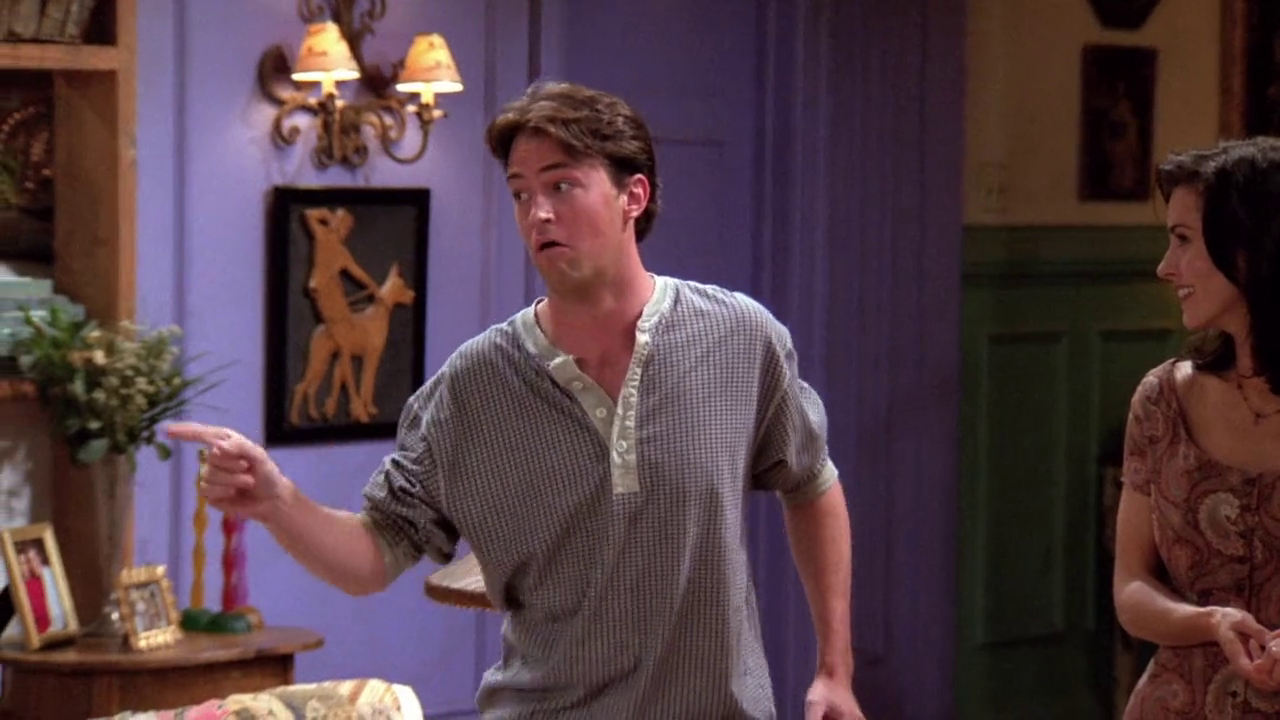
\includegraphics[trim={0 6cm 0 2cm,}, clip, width=\paperwidth]{./S01/img/3/david-hasselhoff.png}
    % \caption{David Hasselhoff\label{fig:david-hasselhoff}}
  \end{adjustwidth}
\end{figure}

\begin{tcolorbox}[enhanced,center upper,
    drop fuzzy shadow southeast, boxrule=0.3pt,
    lower separated=false,
    colframe=black!30!dialogoBorder,colback=white]
\begin{minipage}[c]{0.16\linewidth}
  \raisebox{\dimexpr-\height+\ht\strutbox\relax}{
    \centering 
\includegraphics[width=1.4cm]{./assets/img/chandler.png}
  }
   & \centering \scriptsize{Chandler}
\end{minipage}
\hfill
\begin{minipage}[c]{0.8\linewidth}
  \textbf{- I'd marry him just for his David Hasselhoff impression alone.}\\
  - Eu casaria por causa da imitação de David Hasselholff.
\end{minipage}
\end{tcolorbox}

\emph{David Hasselhoff} é ator, cantor, produtor e empresário
norte-americano. Um de seus grandes papeis de sucesso foi o salva-vidas
\emph{Mitch Buchannon} em \emph{Baywatch} (1989-2001), conhecida no
Brasil como \emph{S.O.S. Malibu}\footnote{\sloppy David Hasselhoff - IMDB. \url{https://www.imdb.com/name/nm0001327/}}
\footnote{\sloppy Site oficial Baywatch. \url{https://www.baywatch.com/}},
série que acaba sendo conhecida como a preferida de Joey no episódio
\textbf{\textcolor{primarycolor}{S03E06 - Aquele do flashback}}, em que
ele apresenta a série a Chandler.

\begin{figure}
  \centering
  \begin{tikzpicture}
    \node [inner sep=0pt] at (0,0) {
      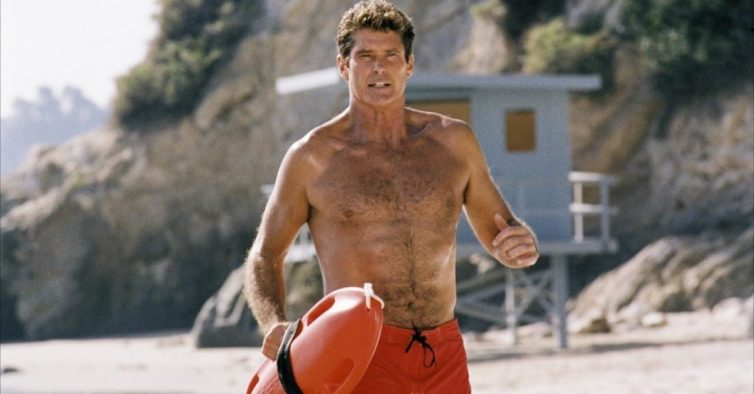
\includegraphics[width=0.7\textwidth,keepaspectratio]{./S01/img/3/david-hasselhoff-baywatch.jpg}
    };
    \draw [white, rounded corners=\ClipSep, line width=\ClipSep]
    (current bounding box.north west) --
    (current bounding box.north east) --
    (current bounding box.south east) --
    (current bounding box.south west) -- cycle
    ;
    \end{tikzpicture}
    \caption{David Hasselhoff em Baywatch\label{fig:david-hasselhoff-em-baywatch}}
\end{figure}

\hypertarget{bugs-bunny}{%
\section{Bugs Bunny}\label{bugs-bunny}}

\begin{figure}[!ht]
  \begin{adjustwidth}{-\oddsidemargin-1in}{-\rightmargin}
    \centering
    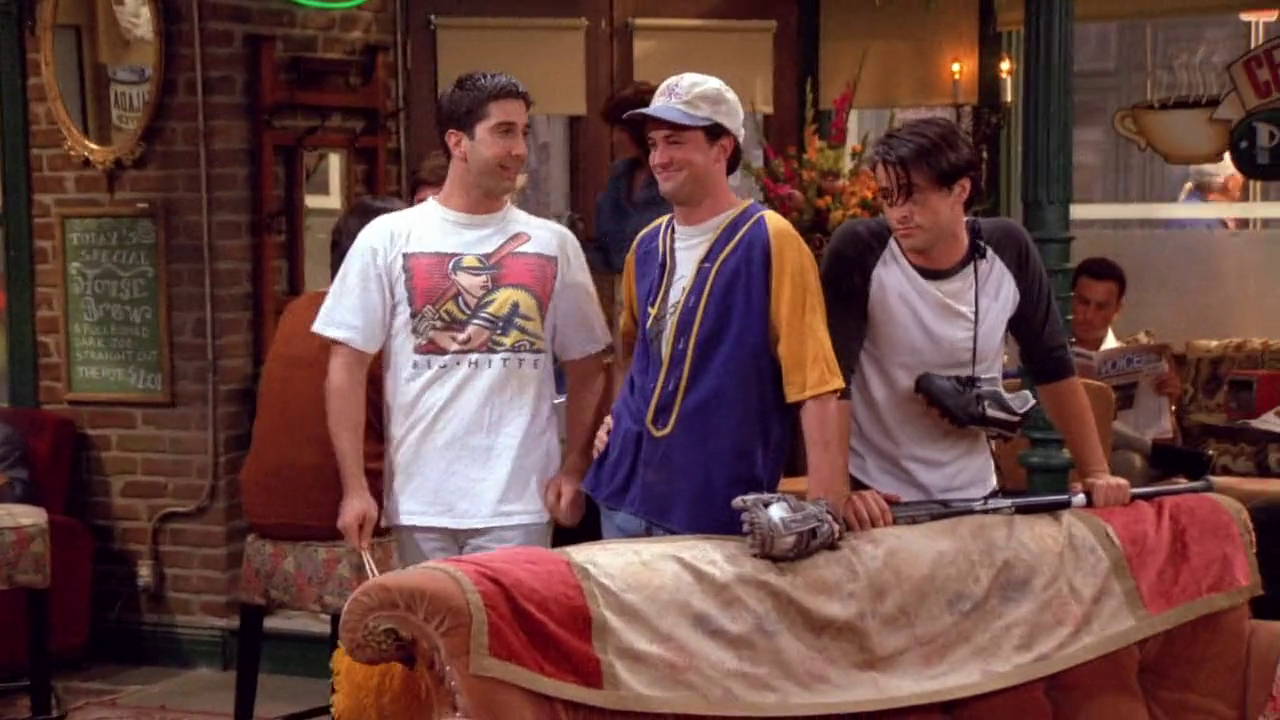
\includegraphics[trim={0 8cm 0 2cm,}, clip, width=\paperwidth]{./S01/img/3/bugs-bunny.png}
    % \caption{Bugs Bunny\label{fig:bugs-bunny}}
  \end{adjustwidth}
\end{figure}

\begin{tcolorbox}[enhanced,center upper,
    drop fuzzy shadow southeast, boxrule=0.3pt,
    lower separated=false, breakable,
    colframe=black!30!dialogoBorder,colback=white]
\begin{minipage}[c]{0.16\linewidth}
  \raisebox{\dimexpr-\height+\ht\strutbox\relax}{
    \centering 
\includegraphics[width=1.4cm]{./assets/img/ross.png}
  }
   & \centering \scriptsize{Ross}
\end{minipage}
\hfill
\begin{minipage}[c]{0.8\linewidth}
  \textbf{- He was like that Bugs Bunny cartoon where Bugs is playing all the positions.}\\
  - Ele parecia o Pernalonga no desenho em que jogava em todas as posições.
\end{minipage}
\end{tcolorbox}

\saveparinfos
\noindent
\begin{minipage}[c]{0.5\textwidth}\useparinfo

Enquanto explica como Alan joga bem \emph{softball} \footnote{\sloppy Diferenças entre softball e baseball (Inglês). \url{https://www.dummies.com/sports/fantasy-sports/fantasy-baseball/the-differences-between-softball-and-baseball/}},
Ross menciona \emph{Bugs Bunny}, conhecido no Brasil como
\emph{Pernalonga}, personagem da \emph{Looney Tunes}. O episódio citado
por Ross é o \emph{Baseball Bugs} (1946).\footnote{\sloppy Baseball Bugs - IMDB. \url{https://www.imdb.com/title/tt0038333/}}
\footnote{\sloppy Baseball Bugs - Episódio na SuperCartoons (Inglês). \url{https://www.supercartoons.net/cartoon/629/bugs-bunny-baseball-bugs.html}}

\end{minipage}\hfill
\begin{minipage}[c]{0.5\textwidth}

\begin{figure}
  \centering
  \begin{tikzpicture}
    \node [inner sep=0pt] at (0,0) {
      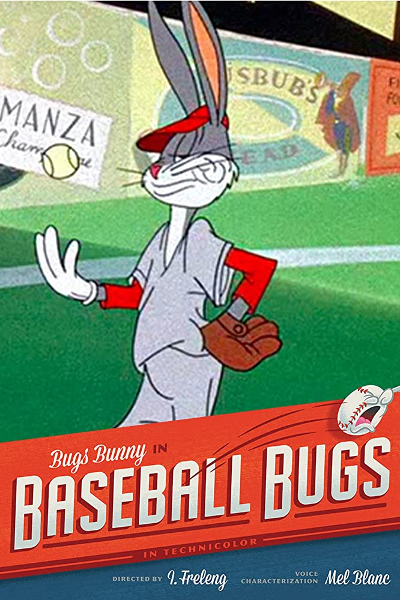
\includegraphics[width=0.6\textwidth,keepaspectratio]{./S01/img/3/baseball-bugs.jpg}
    };
    \draw [white, rounded corners=\ClipSep, line width=\ClipSep]
    (current bounding box.north west) --
    (current bounding box.north east) --
    (current bounding box.south east) --
    (current bounding box.south west) -- cycle
    ;
    \end{tikzpicture}
    \caption{Baseball Bugs\label{fig:baseball-bugs}}
\end{figure}

\end{minipage}

\hypertarget{lamb-chop}{%
\section{Lamb Chop}\label{lamb-chop}}

\begin{figure}[!ht]
  \begin{adjustwidth}{-\oddsidemargin-1in}{-\rightmargin}
    \centering
    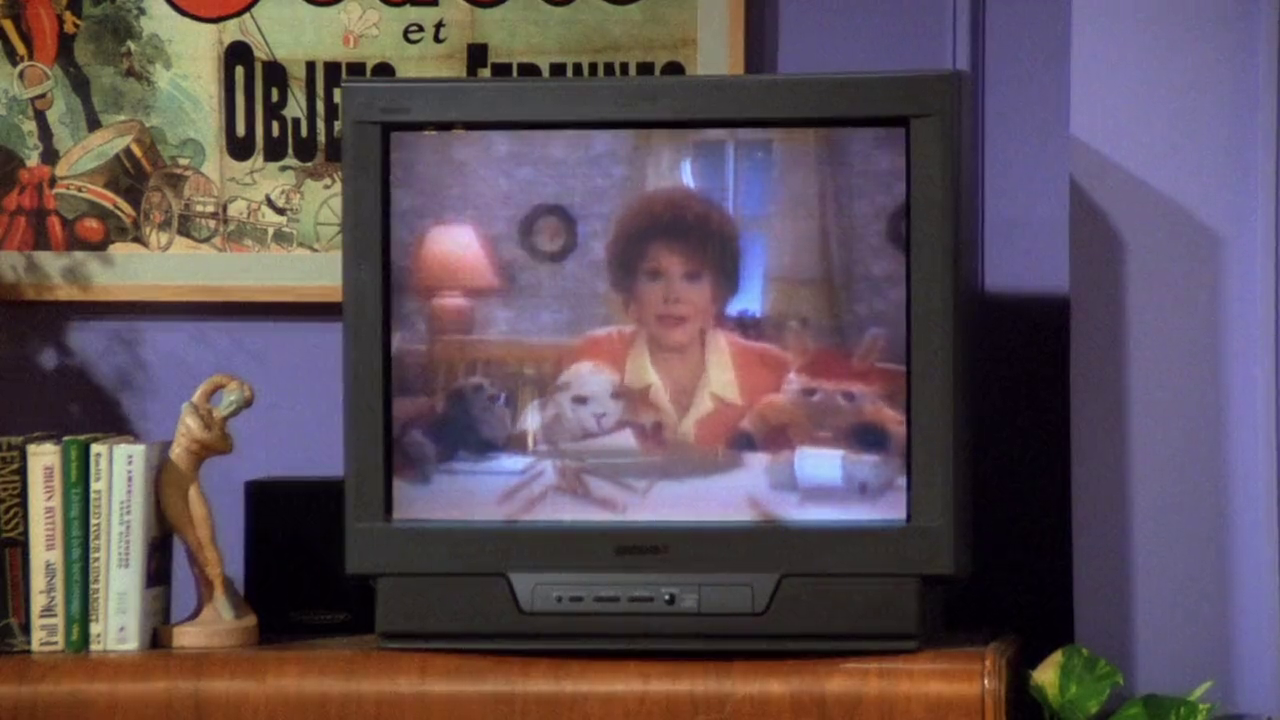
\includegraphics[trim={0 6cm 0 3cm,}, clip, width=\paperwidth]{./S01/img/3/lamb-chop.png}
    % \caption{Lamb Chop\label{fig:lamb-chop}}
  \end{adjustwidth}
\end{figure}

\begin{tcolorbox}[enhanced,center upper,
    drop fuzzy shadow southeast, boxrule=0.3pt,
    lower separated=false, breakable,
    colframe=black!30!dialogoBorder,colback=white]
\begin{minipage}[c]{0.16\linewidth}
  \raisebox{\dimexpr-\height+\ht\strutbox\relax}{
    \centering 
\includegraphics[width=1.4cm]{./assets/img/chandler.png}
  }
   & \centering \scriptsize{Chandler}
\end{minipage}
\hfill
\begin{minipage}[c]{0.8\linewidth}
  \textbf{- If I had a sock on my hand for 30 years, it'd be talking too.}\\
  - Se eu usasse uma meia na mão por 30 anos, ela também ia falar.
\end{minipage}
\end{tcolorbox}

No apartamento de Monica os amigos assistem a \emph{Lamb Chop}, fantoche
criado por \emph{Shari Lewis} (1934-1998). Sua filha, \emph{Mallory
Lewis}, continuou seu legado e faz performances de \emph{Lamb Chop} até
hoje.\footnote{\sloppy Lamb Chop - Site oficial. \url{https://mallorylewisandlambchop.com/faqs/}}

\begin{figure}
  \centering
  \begin{tikzpicture}
    \node [inner sep=0pt] at (0,0) {
      
\includegraphics[width=0.6\textwidth,keepaspectratio]{./S01/img/3/shari-lewis.jpg}
    };
    \draw [white, rounded corners=\ClipSep, line width=\ClipSep]
    (current bounding box.north west) --
    (current bounding box.north east) --
    (current bounding box.south east) --
    (current bounding box.south west) -- cycle
    ;
    \end{tikzpicture}
    \caption{Shari Lewis\label{fig:shari-lewis}}
\end{figure}
